\documentclass[a4paper,12pt]{article}

\usepackage[margin=2.5cm]{geometry}  % change page margins

%%% Работа с русским языком
\usepackage{cmap}					% поиск в PDF
\usepackage{mathtext} 				% русские буквы в формулах
\usepackage[T2A]{fontenc}			% кодировка
\usepackage[utf8]{inputenc}			% кодировка исходного текста
\usepackage[english,russian]{babel}	% локализация и переносы

%%% Дополнительная работа с математикой
\usepackage{amsfonts,amssymb,amsthm,mathtools} % AMS
\usepackage{amsmath}
\usepackage{icomma} % "Умная" запятая: $0,2$ --- число, $0, 2$ --- перечисление

%% Шрифты
\usepackage{euscript} % Шрифт Евклид
\usepackage{mathrsfs} % Красивый матшрифт
\usepackage{pifont}   % Dingbats

\usepackage{relsize}  % for \mathlarger

%% Перенос знаков в формулах (по Львовскому)
\newcommand*{\hm}[1]{#1\nobreak\discretionary{}{\hbox{$\mathsurround=0pt #1$}}{}}

%%% Работа с таблицами
\usepackage{array,tabularx,tabulary,booktabs} % Дополнительная работа с таблицами
\usepackage{longtable}  % Длинные таблицы
\usepackage{multirow}   % Слияние строк в таблице

\usepackage{color}

\usepackage{graphicx,wrapfig,float}
\numberwithin{figure}{section}
\graphicspath{{images-combinat/}}

\usepackage{hyperref}
\hypersetup{
	colorlinks=true,
	linkcolor=blue,
	filecolor=magenta,      
	urlcolor=cyan,
}
%\urlstyle{same}
%\usepackage[stable]{footmisc}   % footnotes in section headings

\theoremstyle{definition}
\newtheorem{definition}{Опр.}[section]
\newtheorem*{property}{Св-во}  %[definition]
%\theoremstyle{plain}
%\theoremstyle{remark}
\theoremstyle{definition}
\newtheorem{theorem}{Tеор.}[section]
\newtheorem*{corollary}{Сл-е} %[theorem]
\newtheorem{lemma}{Лемма}[section]
\renewcommand\qedsymbol{$\blacksquare$}

\def\ilet{$\gimel\;$}
\def\iiff{$\;\Longleftrightarrow\;$}
\def\iiChi{\mathcal{X}}
\def\iiany{$\forall\;$}
\def\iiTODO{\guillemotleft$\mathcal{TODO}$\guillemotright\textellipsis}

%%% Заголовок
\title{Основы дискретной математики.\\Комбинаторика.}
\author{}
\date{}

\begin{document}

\maketitle

\tableofcontents



\section{Определения}


\begin{definition}[Покрытие $\{X_i\}$ множества $X$]
	$\bigcup{X_i} = X$
\end{definition}

\begin{definition}[Разбиение]
	\[\begin{cases}
		& \bigcup{X_i} = X \\
		& X_i \cap X_j = \varnothing \\
		& X_i \ne \varnothing
	\end{cases}\]
\end{definition}

\begin{definition}[Упорядоченное разбиение]  \label{def.ord.break}
	\[\begin{cases}
		& \text{разбиение} \\
		& X_1 \preccurlyeq X_2 \preccurlyeq ... \preccurlyeq X_n
	\end{cases}\]
\end{definition}

\begin{definition}[Разделение]  \label{def.division}
	\[ \begin{cases}
		& \text{``почти'' разбиение} \\
		& X_i \approx \varnothing \\
		& X_1 \preccurlyeq ... \preccurlyeq X_n
	\end{cases} \]
\end{definition}

\begin{definition}[Декартова степень]
	\[ X^k = \{(x_1,...,x_k): \; x_i \in X, \; x_1 \preccurlyeq ... \preccurlyeq x_k \} \]
\end{definition}

\begin{definition}[$k$-мультимножество]
	\[ M_k(X) = \{(x_1,...,x_k): \; x_i \in X, \; x_1 \approx ... \approx x_k \} \]
\end{definition}

\begin{definition}[$k$-мультимножество (2)]
	\begin{align*}
		& M_k = (X, \varphi) \\
		& \varphi: X \rightarrow \overline{0,k} \\
		& \sum{\varphi(x_i)} = k \quad \varphi(x_i) \in \overline{0,k}
	\end{align*}
\end{definition}

\begin{definition}[$k$-сочетание (без повторений)]
	\textit{неупорядоченное} $k$-элементное подмножество $n$-элементного множества
\end{definition}

\begin{definition}[$k$-сочетание с повторениями]
	$\approx$ $k$-мультимножество $\approx$ $k$ монеток в кармане
\end{definition}



\section{Биномиальные коэффициенты}

$\binom{n}{k}$ --- количество неупорядоченных $k$-элементных подмножеств $n$-элементного множества
	\[ \binom{n}{k} = \frac{n(n-1)...(n-k+1)}{k!} = \frac{(n)_k}{k!} \]


\begin{align*}
	\binom{n}{k} &= \frac{n!}{k!(n-k)!} \\
	\binom{n}{k} &= 0 \qquad k > n \\
	\binom{n}{0} &= 1 \qquad n \geqslant 0
\end{align*}

В самом общем виде:
	\[ \binom{q}{k} = \begin{cases*}
		\frac{n(n-1)...(n-k+1)}{k!}, \quad k \in \mathbb{N}, q \in \mathbb{C} \\
		1,  \qquad k=0 \\
		0,  \qquad k<0
	\end{cases*} \]

Рекуррентное свойство:
\[ \binom{n}{k} = \binom{n}{n-k} \]

\begin{figure}[H]
	\centering
	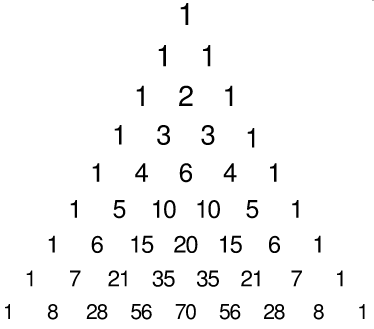
\includegraphics[width=6cm]{pascal-triangle.png}
	\hspace{1cm}
	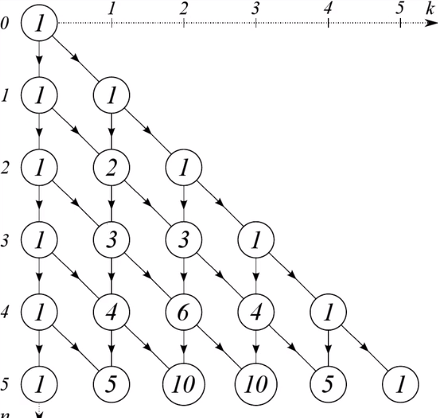
\includegraphics[width=6cm]{pascal-triangle-2.png}
	\caption{Треугольник Паскаля}
\end{figure}

\begin{align*}
	\binom{n}{k} &= \binom{n-1}{k-1} + \binom{n-1}{k}  \qquad \text{или...} \\
	\binom{n+1}{k} &= \binom{n}{k} + \binom{n}{k-1} \\
	\binom{n+m}{k} &= \sum_{i=0}^{k} \binom{n}{i} \binom{m}{k-i} \\
	\binom{2n}{n} &= \sum_{k=0}^{n} {\binom{n}{k}}^2  \qquad \text{
		(\textit{$n$ белых} + \textit{$n$ чёрных шаров}...
		 \quad ``свёртка Вандермонда'')
	}
\end{align*}

\[ \binom{n+1}{k+1} = \sum_{m=k}^ {n}\binom{m}{k}  \qquad
	\text{сначала } k \text{ штук} + x_{n+1}\text{, потом } k + x_n - x_{n+1}
	\text{ итд...} \]



\section{Связь с биномом}

\begin{align*}
	(a+b)^n &= \sum_{k=0}^n \binom{n}{k}a^kb^{n-k} \\
	2^n &= \sum_{k=0}^n\binom{n}{k} \\
	0 &= \sum_{k=0}^n (-1)^k \binom{n}{k}
\end{align*}

Т.е. число всех чётных подмножств равно числу всех нечётных (и равно $2^n / 2$)\footnote{ Комбинаторное доказательство этого факта можно найти \href{http://acadclasses.narod.ru/math/lecture9.htm}{по ссылке}. }:
\[
	\binom{n}{0} + \binom{n}{2} + \binom{n}{4} + ...
	\; = \;
	\binom{n}{1} + \binom{n}{3} + \binom{n}{5} + ...
\]




\section{Сочетания с повторениями}

\newcommand{\mbinom}[2] {
	\left( \!\! \middle( \genfrac{}{}{0pt}{}{#1}{#2} \middle) \!\! \right)
}

\begin{theorem}
	Число способов выбрать с повторениями $k$ элементов из $n$ равно:
	\[ \mbinom{n}{k} = \binom{n+k-1}{k} \]
\end{theorem}

\begin{property}[Принцип биекции]
	$f: X \rightarrow Y$ --- биекция $\implies$ $|X|=|Y|$
\end{property}

\[
	\mbinom{q}{k} = \frac{ q(q+1)...(q+k-1) }{k!} = \frac{ q^{(k)} }{k!}
	\qquad \forall\, q\in\mathbb{C},\; k\in\mathbb{N}
\]



\section{Шары, ящики, перегородки}

Замечание\footnote{ Описание \textit{теории шаров и перегородок} можно найти \href{http://acadclasses.narod.ru/math/lecture9.htm}{по ссылке}. }...

\def\jjc{``$\underbracket{\quad}$''}
\def\jjf{``\textbf{f}''}
\def\jjw{``\textbf{w}''}
\def\iif{\mathrm{f}}
\def\iiw{\mathrm{w}}

\begin{theorem}
	Число способов разложить $n$ одинаковых шаров в $k$ упорядоченных ящиков так, чтобы пустых ящиков не было, равно $\binom{n-1}{k-1}$, причём $n \geqslant k$.
\end{theorem}
\begin{proof}
	Между $k$ ящиками \jjc находятся $k-1$ перегородок \jjf, между которыми закладываются $n$ шаров \jjw. Края конструкции обозначим вертикальными чертами: \[ \big|
		\underbracket{\iiw} \iif \underbracket{\iiw\iiw} \iif 
		\underbracket{\iiw} \iif \underbracket{\iiw\iiw}
	\big| \]
	Шары попадают либо между перегородками, либо между крайними перегородками и краями. Эти места соответствуют ящикам.
	Порядок перегородок не важен, но ящики упорядочены слева направо.
	Поскольку пустые ящики не допускаются, перегородки \jjf \; можно вставлять только между шарами \jjw. Таких мест будет $n-1$. Число способов вставить $k-1$ перегородок между ними будет $\binom{n-1}{k-1}$. При $n-1 < k-1$ получится ноль, отсюда условие $n \geqslant k$.
\end{proof}


\begin{theorem}
	Число способов разложить $n$ одинаковых шаров в $k$ упорядоченных ящиков так, что ящики могут быть пустыми, равно $\binom{n+k-1}{n} = \mbinom{k}{n}$.
\end{theorem}
\begin{proof}
	Между $k$ ящиками \jjc \; находятся $k-1$ перегородок \jjf, между которыми закладываются $n$ шаров \jjw. Края конструкции обозначим вертикальными чертами: \[ \big|
	\underbracket{\quad} \iif \underbracket{\iiw} \iif \iif
	\underbracket{\iiw\iiw\iiw} \iif \underbracket{\iiw}
	\big| \]
	Порядок перегородок не важен, но ящики упорядочены слева направо.
	Теперь допускается \iiany перестановка шаров и перегородок. То есть $n$ шаров и $k-1$ перегородок произвольно расставляются на $n+k-1$ посадочных мест. Число способов расставить шары будет $\binom{n+k-1}{n} = \binom{n+k-1}{k-1}$, после чего перегородки расставляются на оставшиеся места.
\end{proof}


\begin{corollary}
	Есть предметы $n$ различных сортов. Число способов выбрать $k$ предметов, если предметы одного сорта неразличимы (иначе говоря, выбрать \textit{с повторениями} $k$ элементов из $n$) равно $\mbinom{n}{k} = \binom{n+k-1}{k} = \binom{n+k-1}{n-1}$.
\end{corollary}
\begin{proof}
	$k$ предметов -- это ``шары'', а $n$ сортов -- ``ящики'', по которым их раскладываем. Получаем аналог задачи выше, но $n$ и $k$ поменялись местами.
\end{proof}



\section{Перестановки}


\begin{definition}[$k$-перестановка (без повторений)]
	\textit{упорядоченное} $k$-элементное подмножество $(x_1,...x_k)$ $n$-элементного множества $|X|=n$, $x_i \in X$; \\
	также называют $k$-размещением из $n$ элементов; \\
	пример: №№ спортсменов на пьедестале (3-перестановка)
\end{definition}

\begin{definition}[$k$-перестановка с повторениями]
	\iiany элемент декартовой степени $X^k$ $n$-элементного множества $|X|=n$; \\
	пример: № паспорта из 8 цифр $\overline{0..9}$
\end{definition}

\begin{property}
	Число $k$-перестановок с повторениями из $n$ равно $n^k$
\end{property}

\begin{property}
	Число $k$-перестановок без повторений из $n$ равно
	\[ P(n,k) = (n)_k = n(n-1)...(n-k+1) = \frac{n!}{(n-k)!} \]
\end{property}

\[ P(n,k) \Bigr|_{n=k} = P(n,n) = P(n) = P_n = n! \]



\section{Схемы с урнами и ящиками}

\begin{figure}[H]
	\centering
	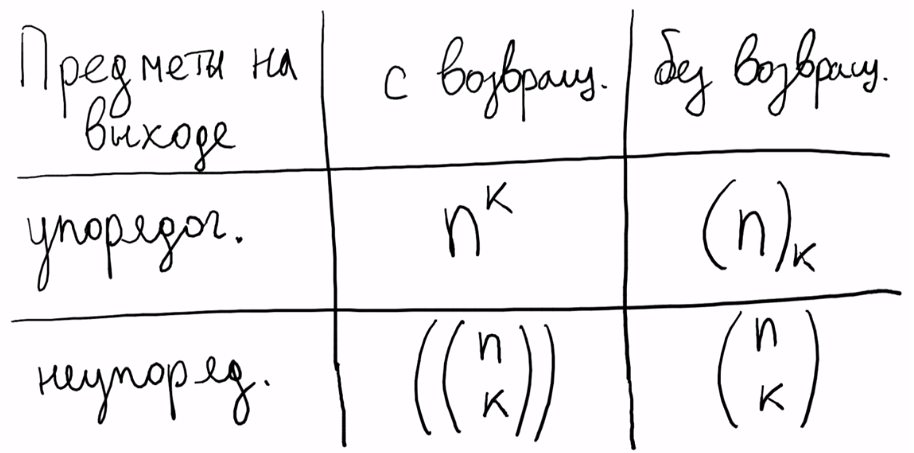
\includegraphics[width=8cm]{schemi-urni.png}
	\caption{Схемы с урнами (\href{https://stepik.org/lesson/9483/step/2}{источник})}
\end{figure}


\begin{figure}[H]
	\centering
	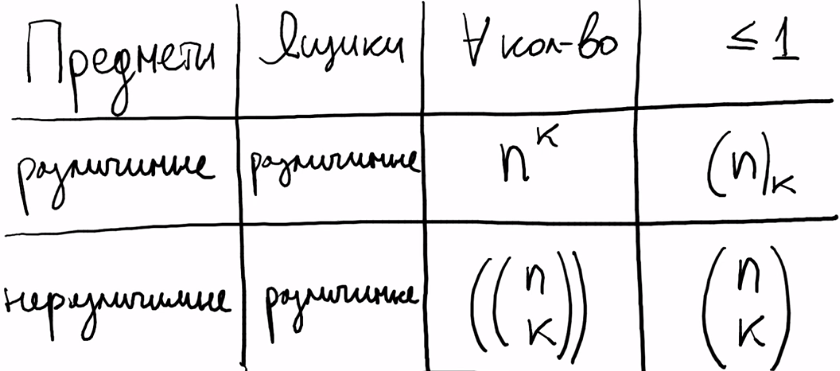
\includegraphics[width=8cm]{schemi-yashiki.png}
	\caption{Cхемы раскладок по ящикам (\href{https://stepik.org/lesson/9483/step/3}{источник})}
\end{figure}


\section{Количество отображений}

\begin{definition}[отображение]
	$x_i \in X \quad f(x_i) \in Y \quad f \in F\quad |X|=n \quad |Y|=k$
\end{definition}

\begin{definition}[инъекция]
	$\forall \; y \in Y: \; |f^{-1}(y) \subseteq X| = \overline{0,1}$
	\qquad  $f(x_1) = f(x_2) \implies x_1 = x_2$
\end{definition}

\begin{definition}[биекция]
	$\forall \; y \in Y \, \exists ! \, f^{-1}(y) \in X$
	\qquad  $f(x_1) = f(x_2) $\iiff$ x_1 = x_2$
\end{definition}

\begin{definition}[сюръекция]
	$\forall \; y \in Y: \; |f^{-1}(y) \subseteq X| > 0$
	\qquad ($\nexists$ если $|X|>|Y|$)
\end{definition}

\begin{align*}
	|\text{отображение}| &= k^n \\
	|\text{инъекция}| &= (k)_n \\
	|\text{биекция}| &= n! \\
	|\text{сюръекция}| &= \hat{S}(n,k)
\end{align*}

\begin{align*}
	\sum_{i=1}^k{ \hat{S}(n,i) \binom{k}{i} } &= k^n   \qquad \text{или...}  \\
   	\sum_{i=0}^n{ \hat{S}(n,i) \binom{k}{i} } &= k^n
   	\qquad \text{т.к. } \hat{S}(n,0)=0, \; \binom{k}{i}\biggr|_{i>k}=0
\end{align*}

используя формулу обращения\footnote{Немного о формулах обращения, например, см. \href{http://iskhacov.narod.ru/materials/combinators.pdf}{здесь}}
\[ f_k = \sum_{i=0}^k{ \binom{k}{i} g_i } \implies
   g_k = \sum_{i=0}^k{ (-1)^{k-i} \binom{k}{i} f_i } \]
получаем
\[ \hat{S}(n,k) = \sum_{i=0}^k{ (-1)^{k-i} \binom{k}{i} i^n }
   \qquad \text{причём } \hat{S}(n,k)\bigr|_{k>n}=0 \]

Отображения $f: X_{|n|} \rightarrow Y_{|k|}$ ``изоморфны'' $\longleftrightarrow$ $k$-разделениям $X$ (\ref{def.division}), $|\{\mathcal{D}_k\}|=k^n$.

Сюръекции $\longleftrightarrow$ упорядоченным $k$-разбиениям $X$ (\ref{def.ord.break}), $|\{\mathcal{B}_k\}|=\hat{S}(n,k)$.



\section{Разделения $\{a_i\}$}

\def\iinfracai{ \frac{n!}{a_1!a_2!...a_k!} }
\def\iisumain{ a_1+...+a_k=n }
\newcommand{\iisubsum}[1]{ {\mathlarger\sum_{\mathclap{\substack{#1}}}} }


\[ P(n;a_1,...,a_k) = \binom{n}{a_1} \cdot \binom{n-a_1}{a_2} \cdot ...
     = \iinfracai   \qquad a_i \geqslant 0, \; \iisumain \]

\begin{align*}
	k^n &= \iisubsum{\iisumain, \\ a_i \geqslant 0} \iinfracai \\
	\hat{S}(n,k) &= \iisubsum{ \iisumain, \\ a_i > 0} \iinfracai
\end{align*}




\vspace{80pt} \noindent \hrulefill~ \raisebox{-8pt}[10pt][10pt]{\Large\ding{102}}~ \hrulefill

\end{document}
